\subsubsection{Mockups}
Für die Erstellung der Mockups wird das Tool Figma verwendet. Innerhalb eines geteilten Workspace werden erste Entwürfe für die fünf verschiedenen Menüs der Applikation erstellt. Damit wird gezeigt, welche Funktionen eine solche App haben soll und wie das Design aussehen könnte.\\

\paragraph{Map}Der Tab „Map“ dient zur Darstellung der verfügbaren Möglichkeiten zur Lagerung von Fahrrädern in der Umgebung auf einer Karte. Mit einem Marker wird ein Fahrradturm dargestellt. Außerdem soll die Verfügbarkeit von freien Plätzen dargestellt werden.\\
\begin{figure}[H]
  \centering
  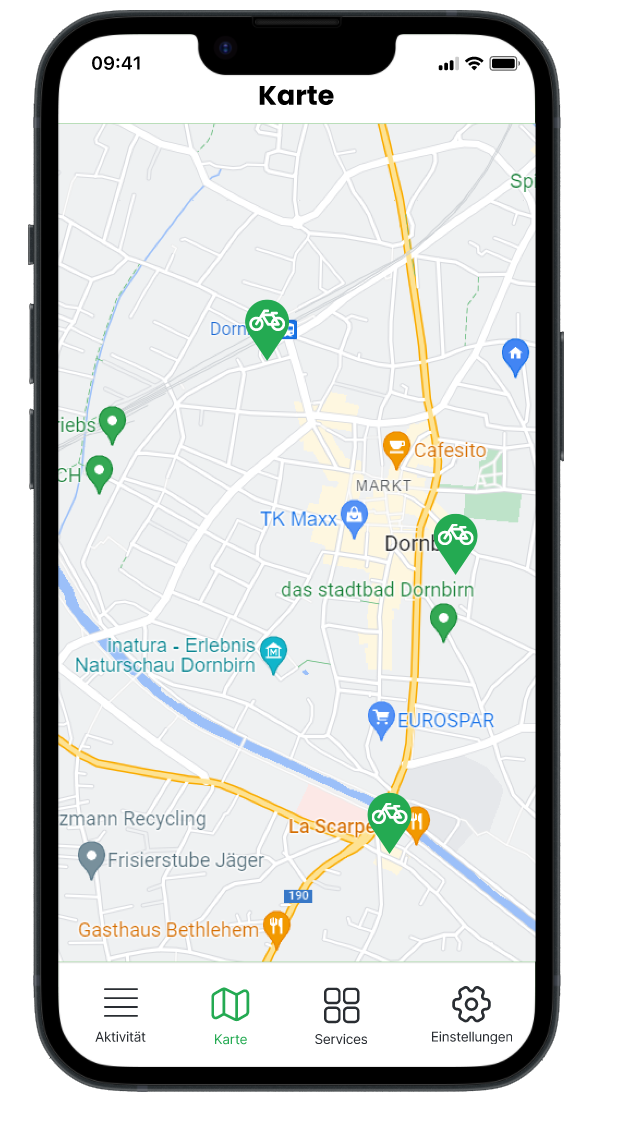
\includegraphics[width=0.2\textwidth]{images/app_mock_map}
  \caption{Mockup vom Screen Map}
  \label{fig:screenmap}
\end{figure}

\paragraph{Tower}Der Tab „Tower“ dient zur Anzeige folgender Informationen:\\
\begin{itemize}
  \item Karte mit Standort des Turmes
  \item Anzahl verfügbaren Lagerungsmöglichkeiten
  \item Bereits von der anwendenden Person bei diesem Turm gelagerte Gegenstände 
  \item Möglichkeit zum Einlagern von einem weiteren Rad oder Gegenstand
\end{itemize}
\begin{figure}[H]
  \centering
  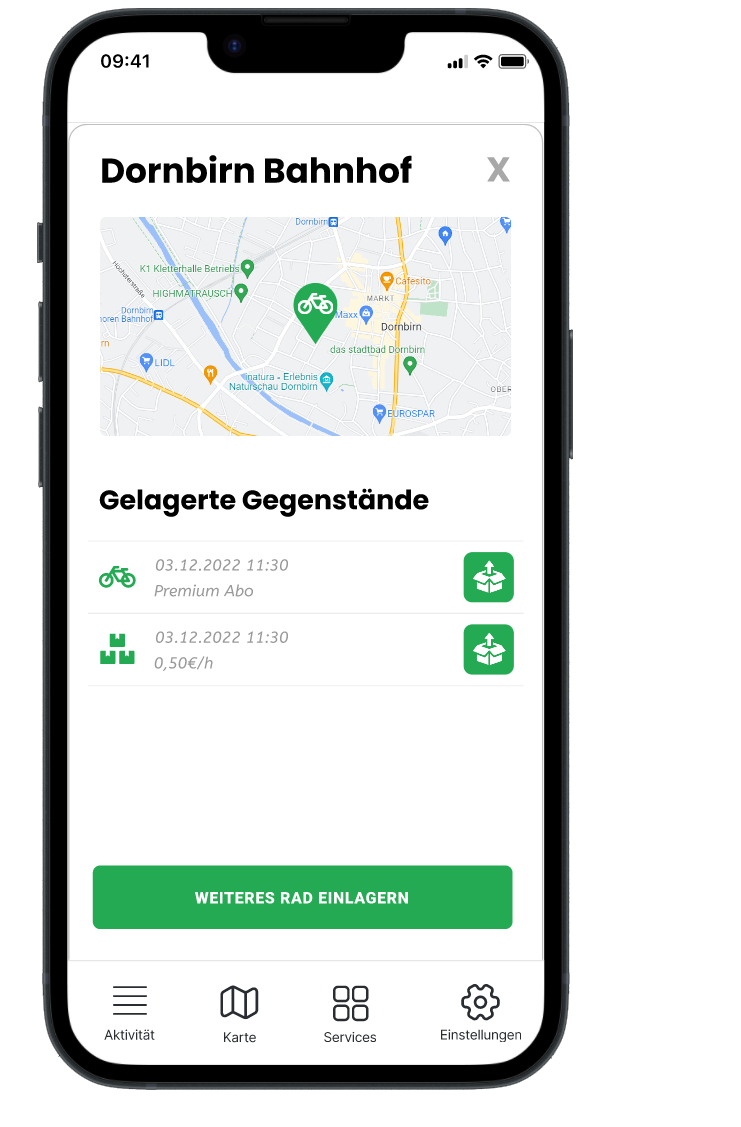
\includegraphics[width=0.2\textwidth]{images/app_mock_tower}
  \caption{Mockup vom Screen Tower}
  \label{fig:screentower}
\end{figure}

\paragraph{Aktivität}Im oberen Teil vom Tab „Aktivität“ werden die von der der anwendenden Person gelagerten Gegenstände angezeigt. Auf der unteren Hälfte werden vergangene Buchungen mit weiteren Informationen aufgelistet. Falls man auf eine Buchung klickt, sollen weitere Infos erscheinen.\\
\begin{figure}[H]
  \centering
  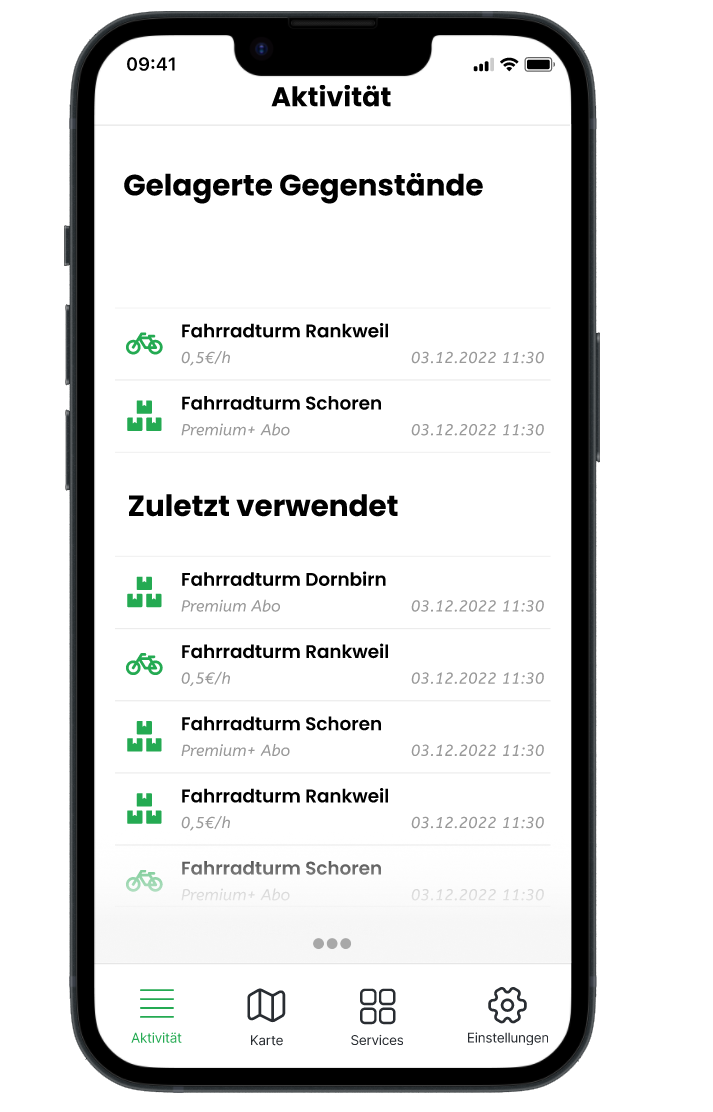
\includegraphics[width=0.2\textwidth]{images/app_mock_objects}
  \caption{Mockup vom Screen Aktivität}
  \label{fig:screenactivity}
\end{figure}

\paragraph{Einstellungen}Der Tab „Einstellungen“ bietet die Möglichkeit zu verschiedenen Unterseiten zu gelangen, wo man wichtige Einstellungen treffen und Informationen abrufen kann.\\
\begin{figure}[H]
  \centering
  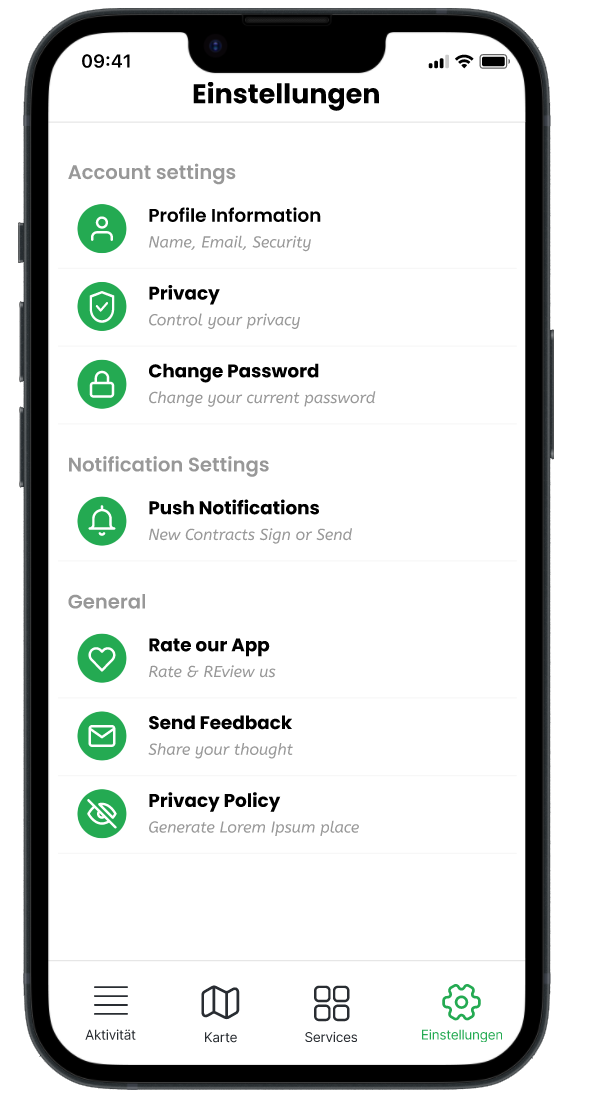
\includegraphics[width=0.2\textwidth]{images/app_mock_settings}
  \caption{Mockup vom Screen Einstellungen}
  \label{fig:screensettings}
\end{figure}

\paragraph{Services}Der Tab „Services“ dient zum Darstellen verschiedener Dienste. Es gibt eine Möglichkeit zum Teilen eines Entsperrungscodes für ein gelagertes Fahrrad und die Eingabe eines solchen Codes. Außerdem werden mehrere externe Dienstleistungsmöglichkeiten zum Beispiel für das Ausleihen eines E-Scooters oder zum Abgeben von Paketen aufgelistet.\\
\begin{figure}[H]
  \centering
  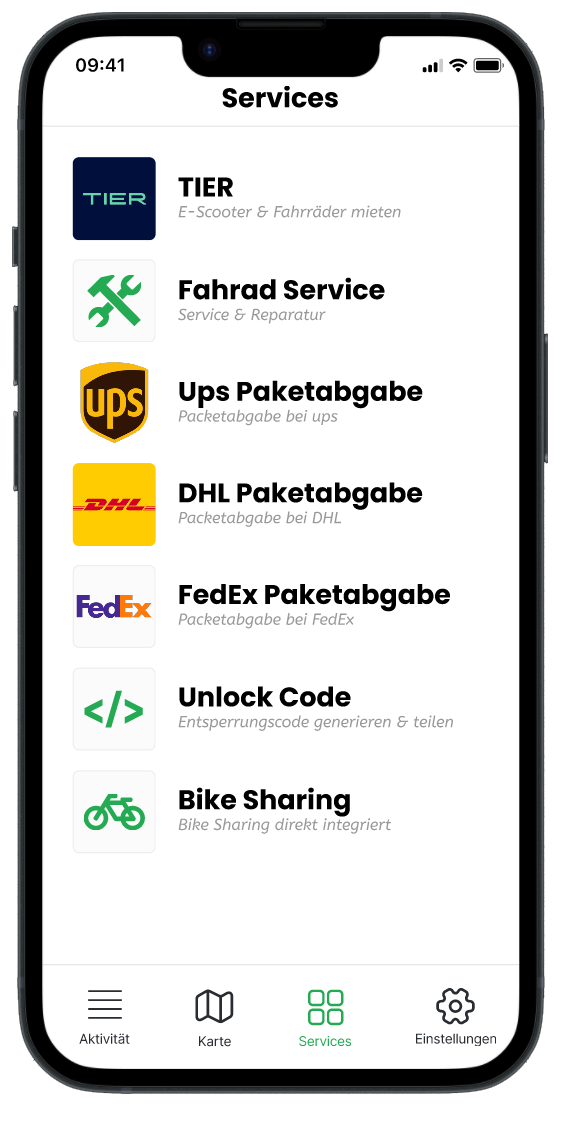
\includegraphics[width=0.2\textwidth]{images/app_mock_services}
  \caption{Mockup vom Screen Services}
  \label{fig:screenservices}
\end{figure}

